\section{}
\[
H(s)=\frac{-1+\j}{\sqrt{2}\,(s+1)^2}\,.
\]
\subsection{Bode-Diagramm}
\begin{center}
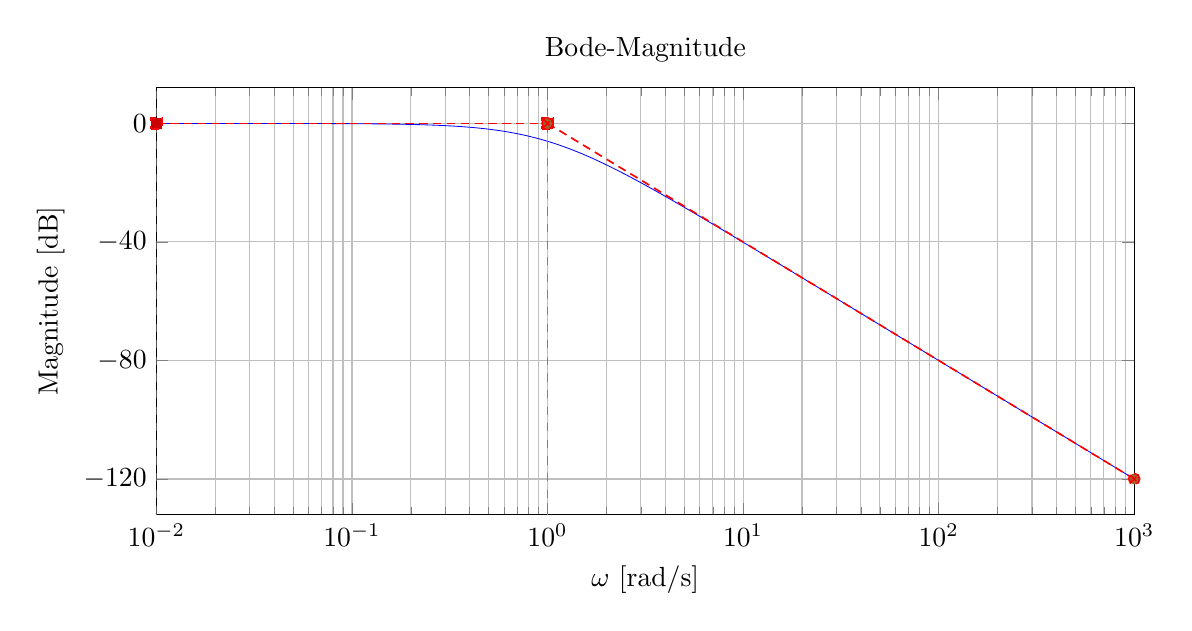
\begin{tikzpicture}
\begin{semilogxaxis}[
  width=14cm,height=7cm,
  xmin=1e-2,xmax=1e3,
  xlabel={$\omega$ [rad/s]},
  ylabel={Magnitude [dB]},
  grid=both,
  ytick distance=40,
  title={Bode-Magnitude}
]
\addplot[
  domain=1e-2:1e3,
  samples=600,
  mark=none,
  line width=0.3pt,
  blue
] {-40*ln(sqrt(1 + x^2))/ln(10)};
\addplot+[domain=1e-2:1,samples=2,dashed,dash pattern=on 3pt off 2pt,line width=0.6pt,red] {0};
\addplot+[domain=1:1e3,samples=2,dashed,dash pattern=on 3pt off 2pt,line width=0.6pt,red] {-40*ln(x)/ln(10)};
\draw[gray,dashed] (rel axis cs:0,0) -- (rel axis cs:0,1);
\draw[gray,dashed] (axis cs:1,\pgfkeysvalueof{/pgfplots/ymin}) -- (axis cs:1,\pgfkeysvalueof{/pgfplots/ymax});
\node[gray,anchor=south east] at (axis cs:1,\pgfkeysvalueof{/pgfplots/ymax}) {\scriptsize Pol $\omega_p=1$ (doppelt)};
\end{semilogxaxis}
\end{tikzpicture}
\vspace{6mm}
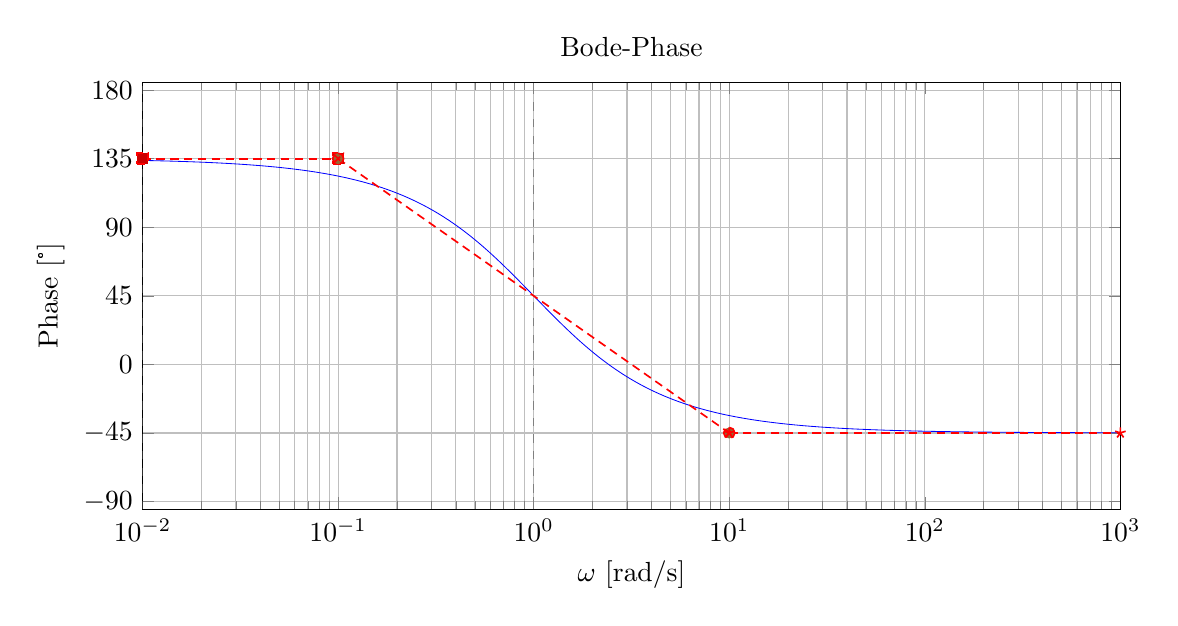
\begin{tikzpicture}
\begin{semilogxaxis}[
  width=14cm,height=7cm,
  xmin=1e-2,xmax=1e3,
  ymin=-95,ymax=185,
  ytick distance=45,
  xlabel={$\omega$ [rad/s]},
  ylabel={Phase [°]},
  grid=both,
  title={Bode-Phase}
]
\addplot[
  domain=1e-2:1e3,
  samples=600,
  mark=none,
  line width=0.3pt,
  blue
] {135 - 2*atan(x)};
\addplot+[domain=1e-2:1e-1,samples=2,dashed,dash pattern=on 3pt off 2pt,line width=0.6pt,red] {135};
\addplot+[domain=1e-1:1e1,samples=2,dashed,dash pattern=on 3pt off 2pt,line width=0.6pt,red] {45 - 90*ln(x)/ln(10)};
\addplot+[domain=1e1:1e3,samples=2,dashed,dash pattern=on 3pt off 2pt,line width=0.6pt,red] {-45};
\draw[gray,dashed] (rel axis cs:0,0) -- (rel axis cs:0,1);
\draw[gray,dashed] (axis cs:1,\pgfkeysvalueof{/pgfplots/ymin}) -- (axis cs:1,\pgfkeysvalueof{/pgfplots/ymax});
\node[gray,anchor=south east] at (axis cs:1,\pgfkeysvalueof{/pgfplots/ymax}) {\scriptsize Pol $\omega_p=1$ (doppelt)};
\end{semilogxaxis}
\end{tikzpicture}
\end{center}
\newpage
\subsection{Erklärung}
\vspace{5mm}
\begin{description}[leftmargin=1.2em,labelsep=.6em,font=\bfseries]
\item[Schritt 1] Konstanter Faktor $(-1+\j)/\sqrt{2}=\mathrm{e}^{\j135^\circ}$: Betrag $1\Rightarrow$ Start bei $0\,\mathrm{dB}$ ohne Anfangssteigung; die Phase "fängt" bei $+135^\circ$ an (reiner Phasor, kein Einfluss auf die Magnitude).
\item[Schritt 2] Doppelpol bei $\omega_p=1\,\mathrm{rad/s}$: ab $\omega=1$ sinkt die Magnitude mit $-40\,\mathrm{dB/dec}$; am Eckpunkt beträgt die exakte Dämpfung $-20\log_{10}(1+1)= -20\log_{10}2\approx-6\,\mathrm{dB}$ (Summe aus zwei $\,-3.01\,\mathrm{dB}$). Die Phase der beiden gleichliegenden Pole fällt zusammen in der Übergangsdekade $\omega\in[0.1,10]$ insgesamt um $180^\circ$; lineare Geradennäherung: $135^\circ\to-45^\circ$ mit $\;\varphi_{\text{approx}}(\omega)=45^\circ-90^\circ\log_{10}\omega$ für $\omega\in[0.1,10]$.
\item[Schritt 3] Grenzverhalten: für $\omega\ll1$ gilt $|H(\j\omega)|_{\mathrm{dB}}\approx0\,\mathrm{dB}$ und $\angle H\approx+135^\circ$ für $\omega\ll0.1$; für $\omega\gg1$ folgt $|H(\j\omega)|_{\mathrm{dB}}\approx-40\log_{10}\omega$ und die Phase nähert sich $+135^\circ-2\cdot90^\circ=-45^\circ$ an.
\end{description}

\vspace{0.5cm}
\medskip
\noindent\textbf{Stückweise Näherung}
\[
|H(\j\omega)|_{\mathrm{dB}}\approx
\begin{cases}
0,& \omega\ll1,\\[4pt]
-20\log_{10}2,& \omega=1,\\[4pt]
-40\log_{10}\omega,& \omega\gg1,
\end{cases}
\qquad
\]
\newpage